\documentclass[11pt,letterpaper]{article}
\usepackage{anysiz_e}
\usepackage{indentfirst}
\usepackage{sectsty}
\usepackage{amsmath}
\usepackage{hyperref}
\usepackage{graphicx}
\usepackage{chngpage}
\usepackage{enumerate}
\hypersetup{
	colorlinks=true, 
	linkcolor=blue, 
	urlcolor=blue, 
	pdfnewwindow=true, 
	citecolor=black
}
\urlstyle{same}
\linespread{1.2}

\begin{document}

\begin{titlepage}
    \vspace*{4cm}
    \begin{flushright}
    {\huge
        Project 3\\[5mm]
    }
    {\large
        CS325 | Spring 2015
     }
    \end{flushright}
\hrule
    \begin{flushright}
	by Group 2\\
	Vedanth Narayanan\\
	Jonathan Merrill\\
	Tracie Lee\\
    \vfill
	\today\\
    \end{flushright}
\end{titlepage}

\raggedright

\section{Transshipment Model}
\subsection*{Part A}


\subsection*{Part B}


\subsection*{Part C}
	

\subsection*{Part D}


\section{Modified from DPV 7.16}
\subsection*{Part A}


\subsection*{Part B}


\subsection*{Part C}


\section{Regression Solution via Linear Programming}
\subsection*{Part A}
\textbf{Objective}: min $\sum\limits_{i=1}^n |y_i -  (a_1x_i + a_0)|$ as an LP.\vspace{8pt}

\textbf{Constraint Equations}

\begin{tabular}{l l l}
$a_0+a_1+z_1\geq3$	&  & $a_0+a_1-z_1\leq3$\\
$a_0+a_1+z_2\geq5$ 	& & $a_0+a_1-z_2\leq5$\\
$a_0+2a_1+z_3\geq13$	& & $a_0+2a_1-z_3\leq13$\\
$a_0+3a_1+z_4\geq8$	& & $a_0+3a_1-z_4\leq8$\\
$a_0+4a_1+z_5\geq10$	& & $a_0+4a_1-z_5\leq10$\\
$a_0+5a_1+z_6\geq14$	& & $a_0+5a_1-z_6\leq14$\\
$a_0+6a_1+z_7\geq18$	& & $a_0+6a_1-z_7\leq18$\\
\end{tabular}\vspace{8pt}

%\textbf{LAD equation}: $y = 2.6x + 2.4$\vspace{8pt}

\textbf{Sum of absolute deviations}: 13.8\vspace{8pt}


\centerline{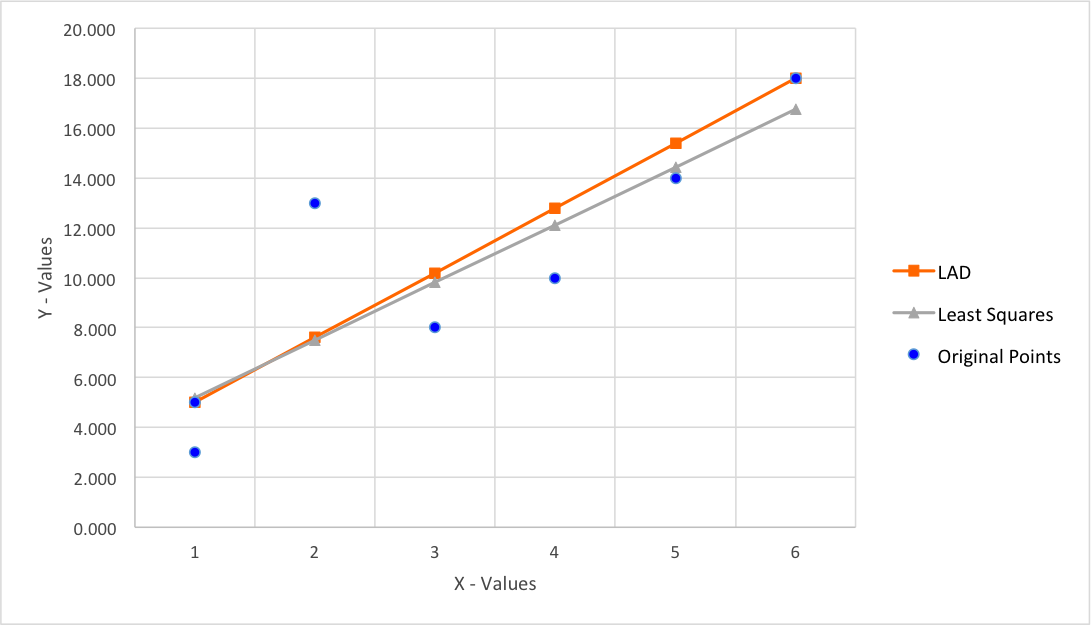
\includegraphics[width=7in]{lad.png}}

This was calculated in Lindo using the constraint equations listed above to obtain the LAD equation $y = 2.6x + 2.4$. In this case, the LAD is close to the original Least Squares solution, especially for x-values close to 0. It appears that as the value of x grows, the gap between the 2 lines will widen.

\subsection*{Part B}
\textbf{Objective}: min $max |y_i -  (a_1x_i + a_0)|$ as an LP.\vspace{8pt}

\textbf{Constraint Equations}

\begin{tabular}{l l l}
$a_0+a_1+z\geq3$		&  & $a_0+a_1-z\leq3$\\
$a_0+a_1+z\geq5$ 		& & $a_0+a_1-z\leq5$\\
$a_0+2a_1+z\geq13$	& & $a_0+2a_1-z\leq13$\\
$a_0+3a_1+z\geq8$		& & $a_0+3a_1-z\leq8$\\
$a_0+4a_1+z\geq10$	& & $a_0+4a_1-z\leq10$\\
$a_0+5a_1+z\geq14$	& & $a_0+5a_1-z\leq14$\\
$a_0+6a_1+z\geq18$	& & $a_0+6a_1-z\leq18$\\
\end{tabular}\vspace{8pt}

%\textbf{MMAD equation}: $y = 2.3x + 4.5$\vspace{8pt}

\textbf{min of the max absolute deviations}: 3.8333\vspace{8pt}

\centerline{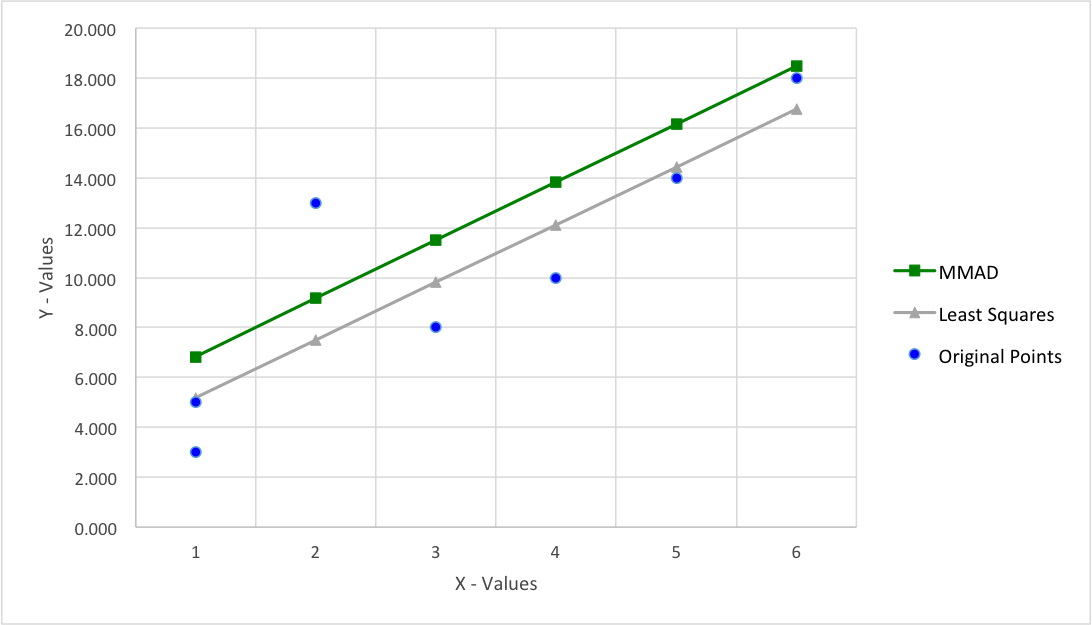
\includegraphics[width=7in]{mmad.png}}

This was calculated again in LIndo using the constraint equations above to obtain the MMAD equation $y = 2.3x + 4.5$. By contrast, the MMAD parallels the Least Squares by almost a full y-value above the Least Squares line. This makes sense since we are merely optimizing or taking the minimum of the maximum possible deviation.\vspace{8pt}



\subsection*{Part C}
\textbf{Objective}: min $\sum\limits_{i=1}^n |y_i -  (a_2x_{2i} + a_1x_{1i} + a_0)|$ as an LP.\vspace{8pt}

\textbf{Constraint Equations}

\begin{tabular}{l l l}
$a_2 + a_1 + a_0 + z_1 \geq 5$ & & $a_2 + a_1 + a_0 - z_1 \leq 5$\\
$2a_2 + a_1 + a_0 + z_2 \geq 9$ & & $2a_2 + a_1 + a_0 - z_2 \leq 9$\\
$2a_2 + 2a_1 + a_0 + z_3 \geq 12$ & & $2a_2 + 2a_1 + a_0 - z_3 \leq 12$\\
$a_2 + 0a_1 + a_0 + z_4 \geq 3$ & & $a_2 + 0a_1 + a_0 - z_4 \leq 3$\\
$0a_2 + 0a_1 + a_0 + z_5 \geq 0$ & & $0a_2 + 0a_1 + a_0 - z_5 \leq 0$\\
$3a_2 + a_1 + a_0 + z_6 \geq 11$ & & $3a_2 + a_1 + a_0 - z_6 \leq 11$\\
\end{tabular}\vspace{8pt}

This was again calculated in Lindo using the constraint equations above to obtain the LAD equation $y = 3x_2 + 3x_1$.

\end{document}
